\begin{comment}
\documentclass[10pt]{article}
\usepackage{fullpage, graphicx, url}
\setlength{\parskip}{1ex}
\setlength{\parindent}{0ex}
\title{grain2}
\begin{document}


\begin{tabular}{ccc}
The Alternative Csound Reference Manual & & \\
Previous & &Next

\end{tabular}

%\hline 
\end{comment}
\section{grain2}
grain2�--� Easy-to-use granular synthesis texture generator. \subsection*{Description}


  Generate granular synthesis textures. \emph{grain2}
 is simpler to use, but \emph{grain3}
 offers more control. 
\subsection*{Syntax}


 ar \textbf{grain2}
 kcps, kfmd, kgdur, iovrlp, kfn, iwfn [, irpow] [, iseed] [, imode]
\subsection*{Initialization}


 \emph{iovrlp}
 -- (fixed) number of overlapping grains. 


 \emph{iwfn}
 -- function table containing window waveform (Use GEN20 to calculate iwfn). 


 \emph{irpow}
 (optional, default=0) -- this value controls the distribution of grain frequency variation. If irpow is positive, the random distribution (x is in the range -1 to 1) is 


 abs(x)�\^{}�((1�/�irpow)�-�1)
; for negative irpow values, it is 

 (1�-�abs(x))�\^{}�((-1�/�irpow)�-�1)
. Setting irpow to -1, 0, or 1 will result in uniform distribution (this is also faster to calculate). The image below shows some examples for irpow. The default value of irpow is 0. 

 


 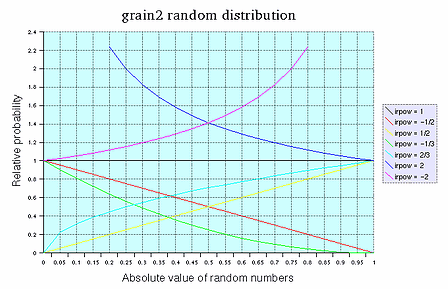
\includegraphics[scale=1]{grain2_rand-448x289} 


 A graph of distributions for different values of irpow.


 \emph{iseed}
 (optional, default=0) -- seed value for random number generator (positive integer in the range 1 to 2147483646 (2 \^{} 31 - 2)). Zero or negative value seeds from current time (this is also the default). 


 \emph{imode}
 (optional default=0) -- sum of the following values: 


 
\begin{itemize}
\item 

 \emph{8:}
 interpolate window waveform (slower).

\item 

 \emph{4:}
 do not interpolate grain waveform (fast, but lower quality).

\item 

 \emph{2:}
 grain frequency is continuously modified by \emph{kcps}
 and \emph{kfmd}
 (by default, each grain keeps the frequency it was launched with). This may be slower at high control rates.

\item 

 \emph{1:}
 skip initialization.


\end{itemize}


 


 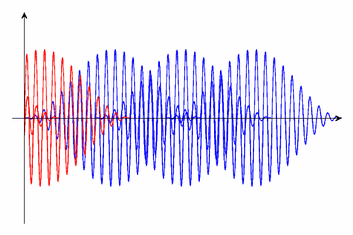
\includegraphics[scale=1]{grain3_2} 


 A diagram showing grains with a start time less than zero in red.
\subsection*{Performance}


 \emph{ar}
 -- output signal. 


 \emph{kcps}
 -- grain frequency in Hz. 


 \emph{kfmd}
 -- random variation (bipolar) in grain frequency in Hz. 


 \emph{kgdur}
 -- grain duration in seconds. \emph{kgdur}
 also controls the duration of already active grains (actually the speed at which the window function is read). This behavior does not depend on the \emph{imode}
 flags. 


 \emph{kfn}
 -- function table containing grain waveform. Table number can be changed at k-rate (this is useful to select from a set of band-limited tables generated by GEN30, to avoid aliasing). 


 


\begin{tabular}{cc}
\textbf{Note}
 \\
� &

 \emph{grain2}
 internally uses the same random number generator as \emph{rnd31}
. So reading \emph{its documentation}
 is also recommended. 


\end{tabular}

\subsection*{Examples}


  Here is an example of the grain2 opcode. It uses the files \emph{grain2.orc}
 and \emph{grain2.sco}
. 


 \textbf{Example 1. Example of the grain2 opcode.}

\begin{lstlisting}
/* grain2.orc */
sr	=  48000
kr	=  750
ksmps	=  64
nchnls	=  2

/* square wave */
i_	ftgen 1, 0, 4096, 7, 1, 2048, 1, 0, -1, 2048, -1
/* window */
i_	ftgen 2, 0, 16384, 7, 0, 4096, 1, 4096, 0.3333, 8192, 0
/* sine wave */
i_	ftgen 3, 0, 1024, 10, 1
/* room parameters */
i_	ftgen 7, 0, 64, -2, 4, 50, -1, -1, -1, 11,			\
			    1, 26.833, 0.05, 0.85, 10000, 0.8, 0.5, 2,	\
			    1,  1.753, 0.05, 0.85,  5000, 0.8, 0.5, 2,	\
			    1, 39.451, 0.05, 0.85,  7000, 0.8, 0.5, 2,	\
			    1, 33.503, 0.05, 0.85,  7000, 0.8, 0.5, 2,	\
			    1, 36.151, 0.05, 0.85,  7000, 0.8, 0.5, 2,	\
			    1, 29.633, 0.05, 0.85,  7000, 0.8, 0.5, 2

ga01	init 0

/* generate bandlimited square waves */

i0	=  0
loop1:
imaxh	=  sr / (2 * 440.0 * exp (log(2.0) * (i0 - 69) / 12))
i_	ftgen i0 + 256, 0, 4096, -30, 1, 1, imaxh
i0	=  i0 + 1
	if (i0 < 127.5) igoto loop1

	instr 1

p3	=  p3 + 0.2

/* note velocity */
iamp	=  0.0039 + p5 * p5 / 16192
/* vibrato */
kcps	oscili 1, 8, 3
kenv	linseg 0, 0.05, 0, 0.1, 1, 1, 1
/* frequency */
kcps	=  (kcps * kenv * 0.01 + 1) * 440 * exp(log(2) * (p4 - 69) / 12)
/* grain ftable */
kfn	=  int(256 + 69 + 0.5 + 12 * log(kcps / 440) / log(2))
/* grain duration */
kgdur	port 100, 0.1, 20
kgdur	=  kgdur / kcps

a1	grain2 kcps, kcps * 0.02, kgdur, 50, kfn, 2, -0.5, 22, 2
a1	butterlp a1, 3000
a2	grain2 kcps, kcps * 0.02, 4 / kcps, 50, kfn, 2, -0.5, 23, 2
a2	butterbp a2, 12000, 8000
a2	butterbp a2, 12000, 8000
aenv1	linseg 0, 0.01, 1, 1, 1
aenv2	linseg 3, 0.05, 1, 1, 1
aenv3	linseg 1, p3 - 0.2, 1, 0.07, 0, 1, 0

a1	=  aenv1 * aenv3 * (a1 + a2 * 0.7 * aenv2)

ga01	=  ga01 + a1 * 10000 * iamp

	endin

/* output instr */

	instr 81

i1	=  0.000001
aLl, aLh, aRl, aRh	spat3di ga01 + i1*i1*i1*i1, 3.0, 4.0, 0.0, 0.5, 7, 4
ga01	=  0
aLl	butterlp aLl, 800.0
aRl	butterlp aRl, 800.0

	outs aLl + aLh, aRl + aRh

	endin
/* grain2.orc */
        
\end{lstlisting}
\begin{lstlisting}
/* grain2.sco */
t 0 60

i 1 0.0 1.3 60 127
i 1 2.0 1.3 67 127
i 1 4.0 1.3 64 112
i 1 4.0 1.3 72 112

i 81 0 6.4

e
/* grain2.sco */
        
\end{lstlisting}
\subsection*{See Also}


 \emph{grain3}

\subsection*{Credits}


 


 


\begin{tabular}{c}
Author: Istvan Varga

\end{tabular}



 


 New in version 4.15


 Updated April 2002 by Istvan Varga
%\hline 


\begin{comment}
\begin{tabular}{lcr}
Previous &Home &Next \\
grain &Up &grain3

\end{tabular}


\end{document}
\end{comment}
